\subsection{Distributed footing: Poroelastic cube (3D) with dynamic consolidation}
Considering the same problem design as the previous section, the mechanical calculation is now extended to allow for time-dependent deformation. In other words, solid displacements are no longer solved to equilibrium, so that solid velocity may be non-zero following solution of the mechanical system.

\subsubsection*{Definition}
All stresses and pressure are zero at the beginning of deformation. Strip
loading ($\sigma_{yy}=\sigma_0$ in $x\in[0,1]$), zero stresses
($\sigma_{yy}=\sigma_{xy}=0$ in $x\in(1,8]$) and zero pressure at
the top; no horizontal flux, no horizontal displacements and zero
shear stresses at left and right hand sides; no vertical flux and no
displacements at bottom (Figure \ref{fig-setting}).

Material parameters are given in Table \ref{tab:mat-dynam}.

\begin{table}[!htb]
\begin{center}
\begin{tabular}{lll}
\hline{\smallskip}
Property & Value & Unit \\
\hline
Young's modulus & $3\times 10^{4}$  & $N/m^{2}$ \\
Poisson's ratio & $0.2, 0.4$       & $-$ \\
Permeability    & $10^{-10}$        & $m^2$ \\
Fluid viscosity & $10^{-3}$         & $Pa\,s$ \\
\hline
\end{tabular}
\end{center}
\caption{Material properties of dynamic consolidation problem.}
\label{tab:mat-dynam}
\end{table}

\subsubsection*{Results}
Time duration is ten time steps. The following figures, Fig. \ref{fig_dynHM1}--\ref{fig_dynHM4} show the distribution of state variables within the domain after 10 time steps. Such distribution is similar to the static case illustrated in Fig. \ref{fig:e10}.
 
\begin{figure}[!htb]
\begin{center}
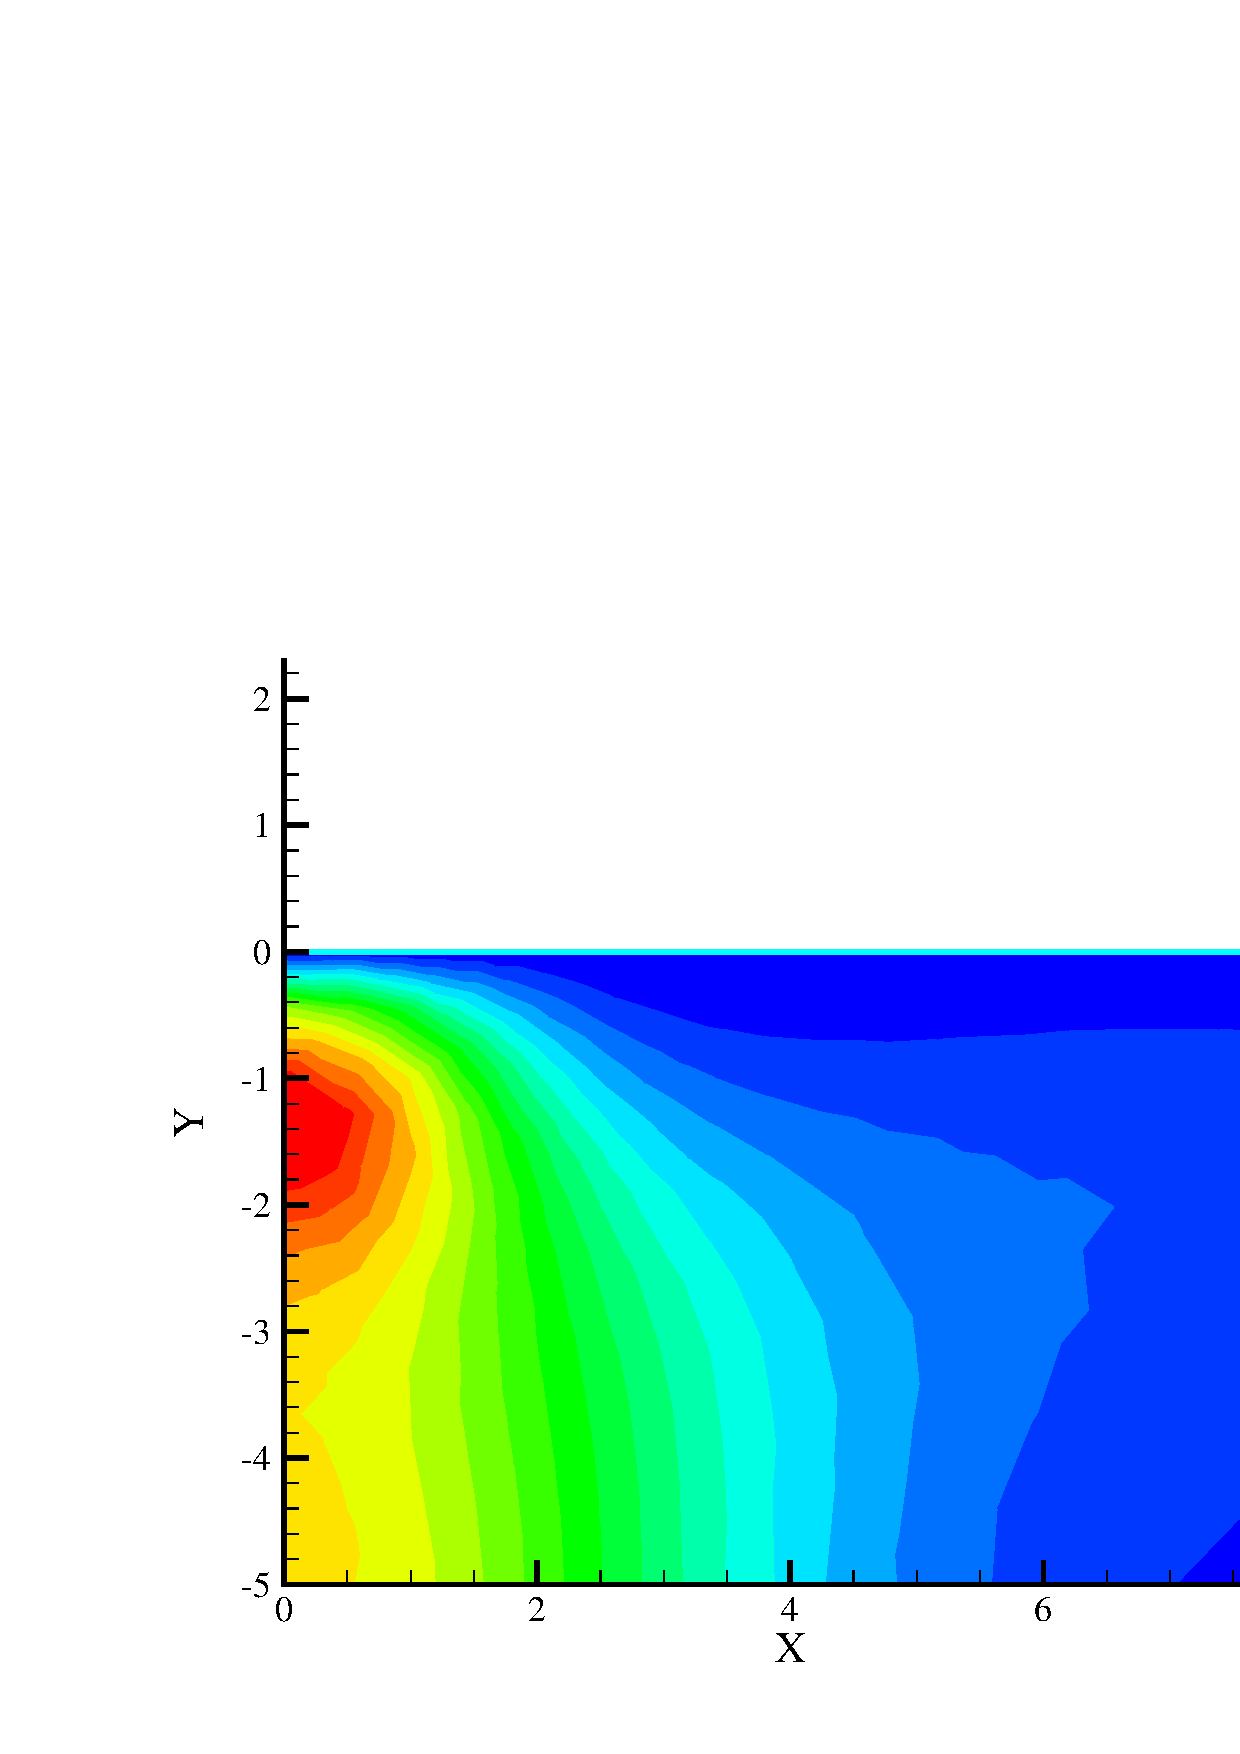
\includegraphics[width=0.49\textwidth]{chapter_14/figures/fig_14_1_8_a}
\includegraphics[width=0.49\textwidth]{chapter_14/figures/fig_14_1_8_b}
\end{center}
\caption{Fluid pressures $p$ and rate of fluid pressure $\dot p$ }
\label{fig_dynHM1}
\end{figure}

\begin{figure}[!htb]
\begin{center}
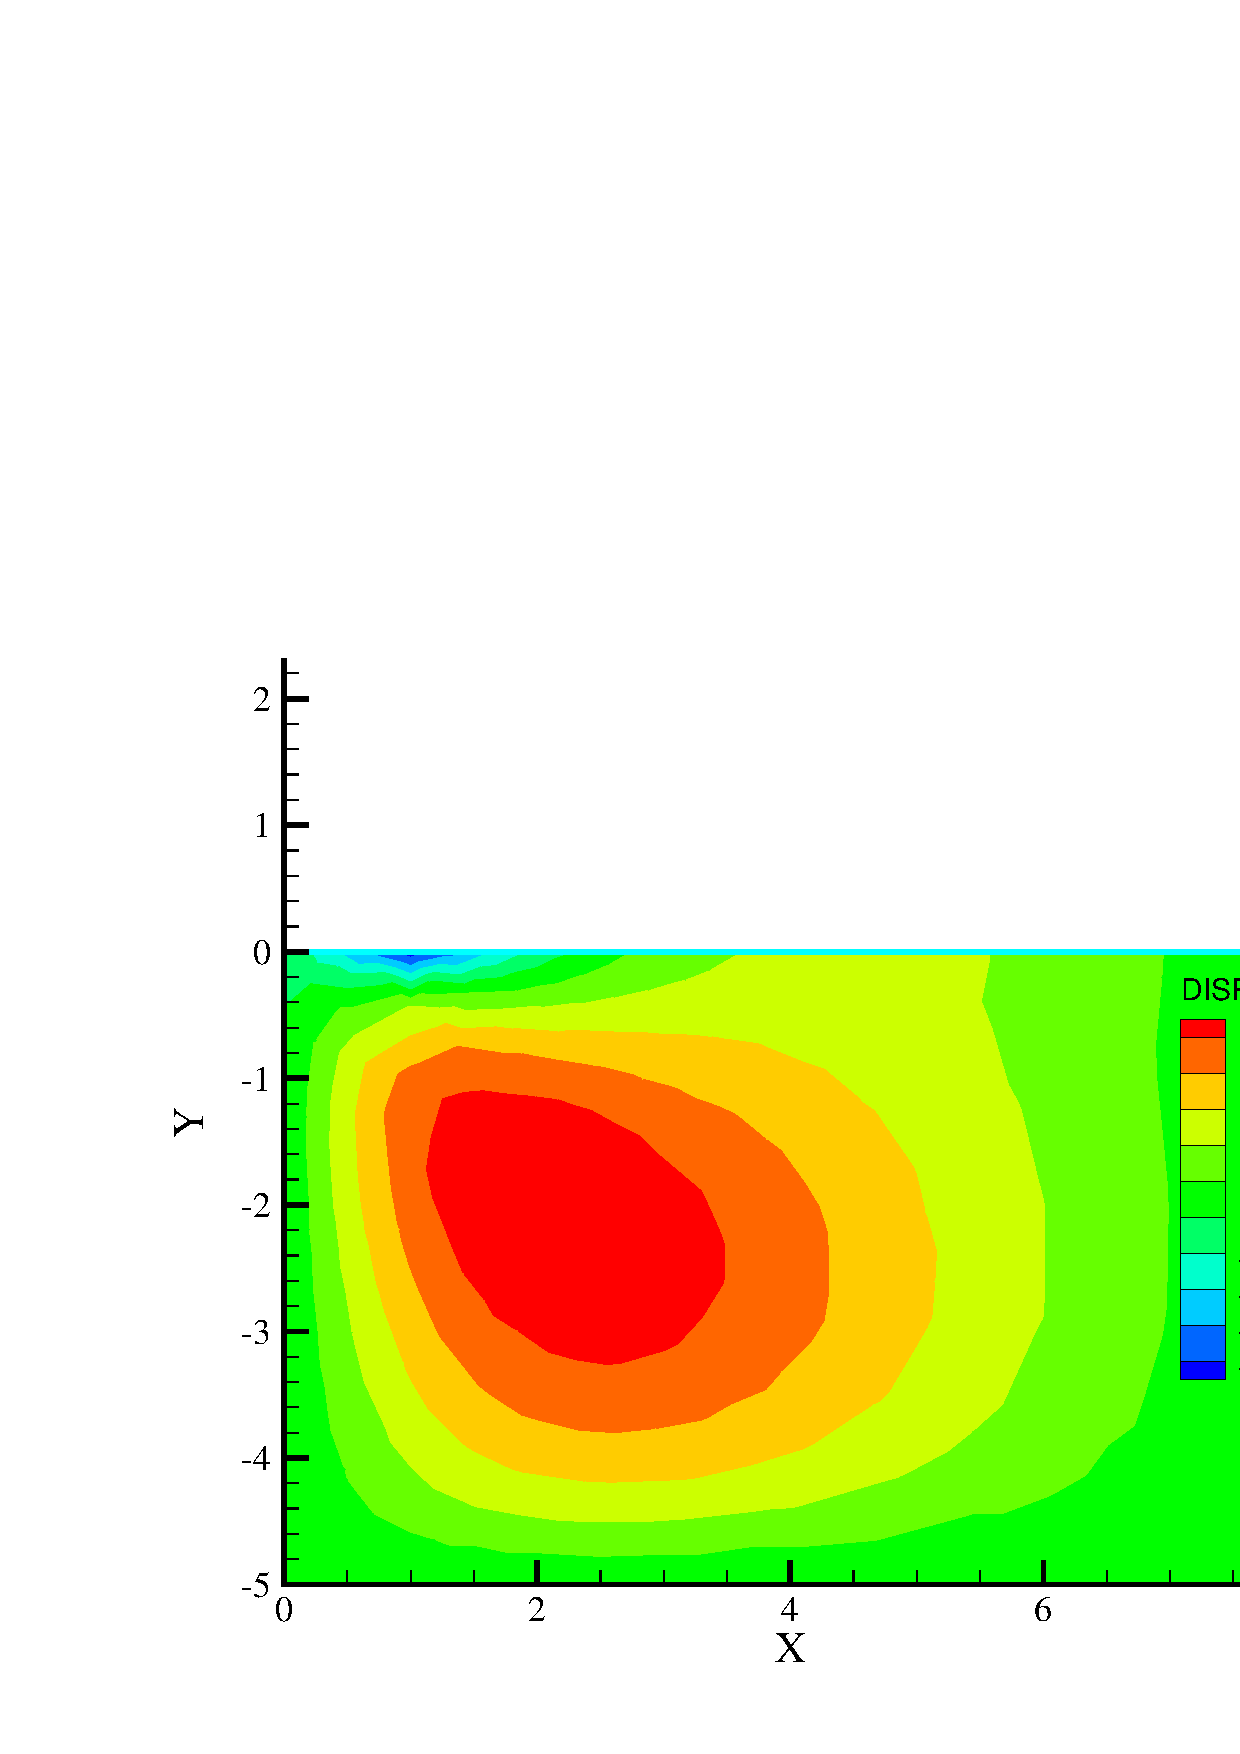
\includegraphics[width=0.32\textwidth]{chapter_14/figures/fig_14_1_9_a}
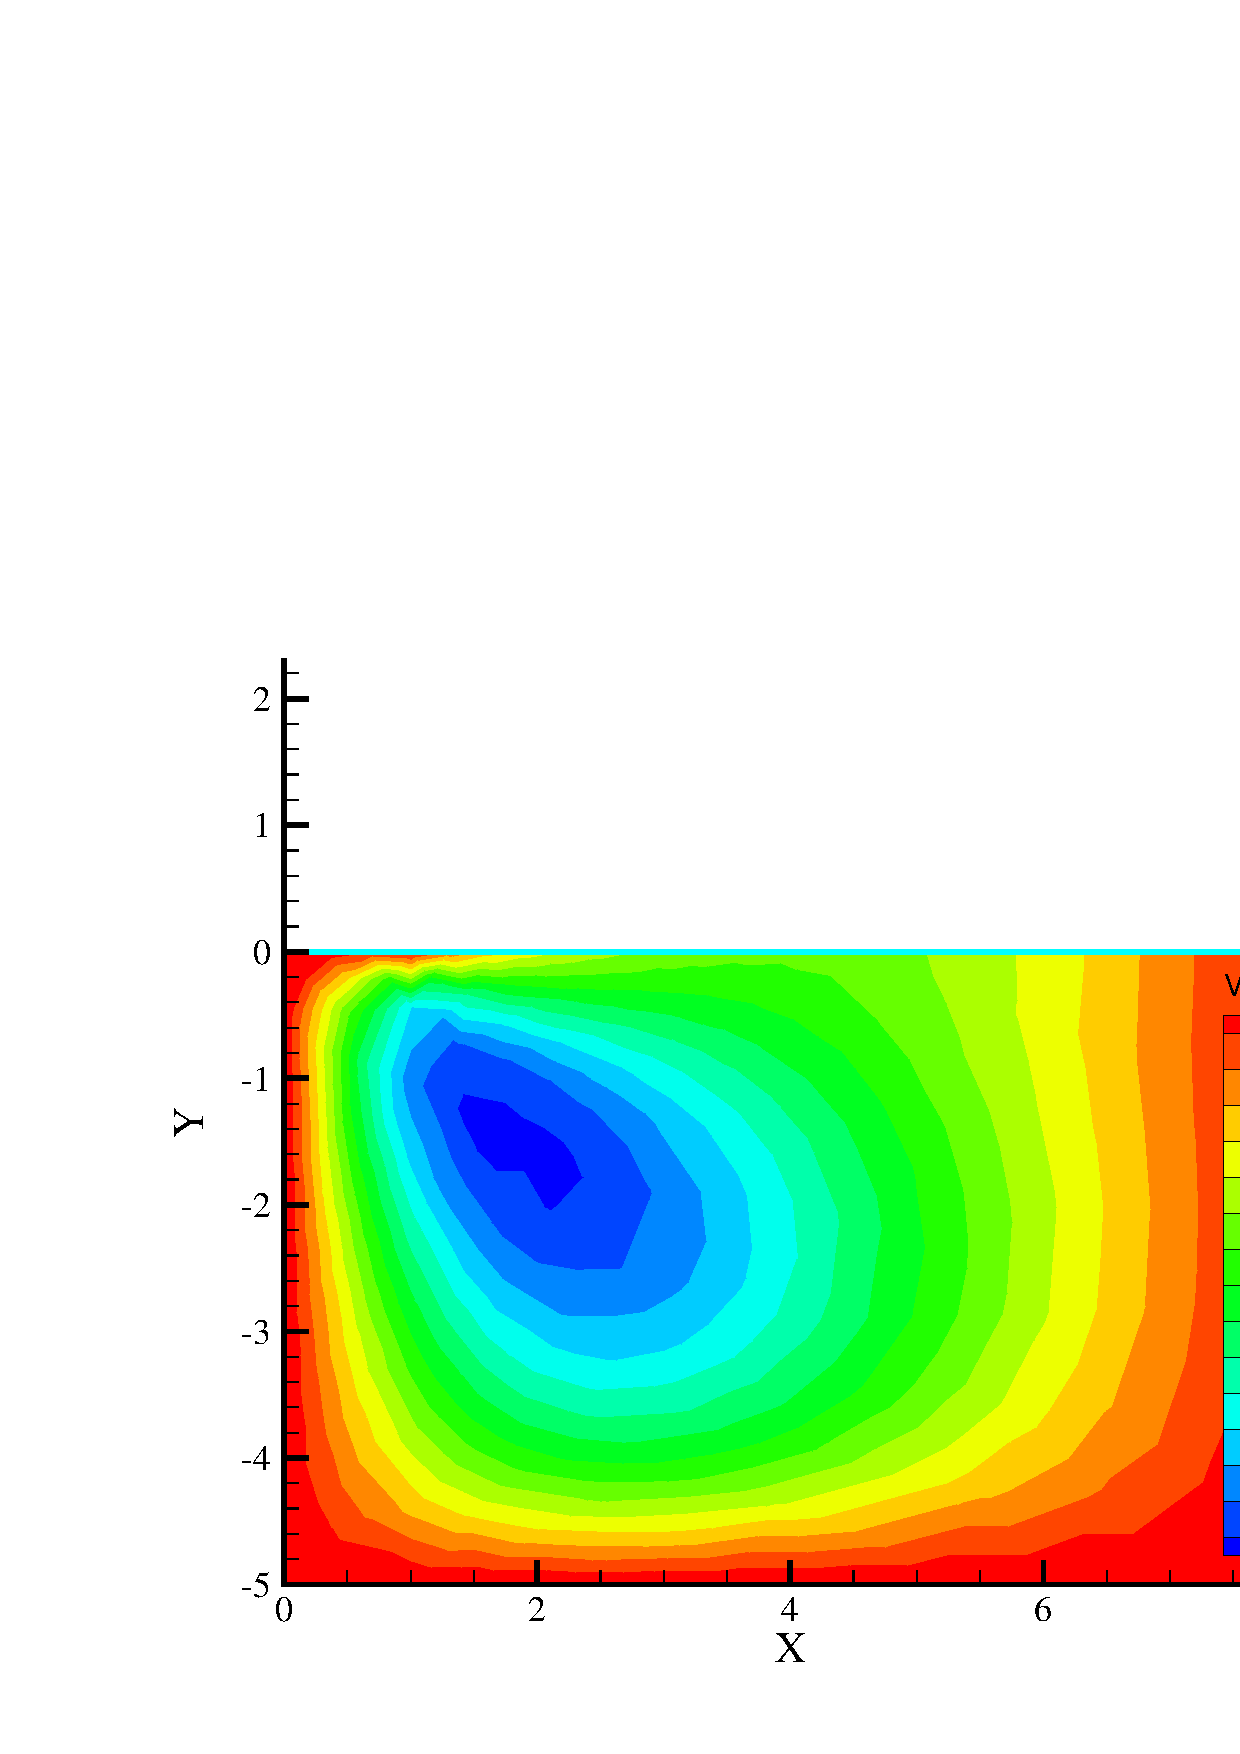
\includegraphics[width=0.32\textwidth]{chapter_14/figures/fig_14_1_9_b}
\includegraphics[width=0.32\textwidth]{chapter_14/figures/fig_14_1_9_c}
\end{center}
\caption{Displacement, its rate and acceleration: horizontal component}
\label{fig_dynHM2}
%\end{figure}
%\begin{figure}[!htb]
\begin{center}
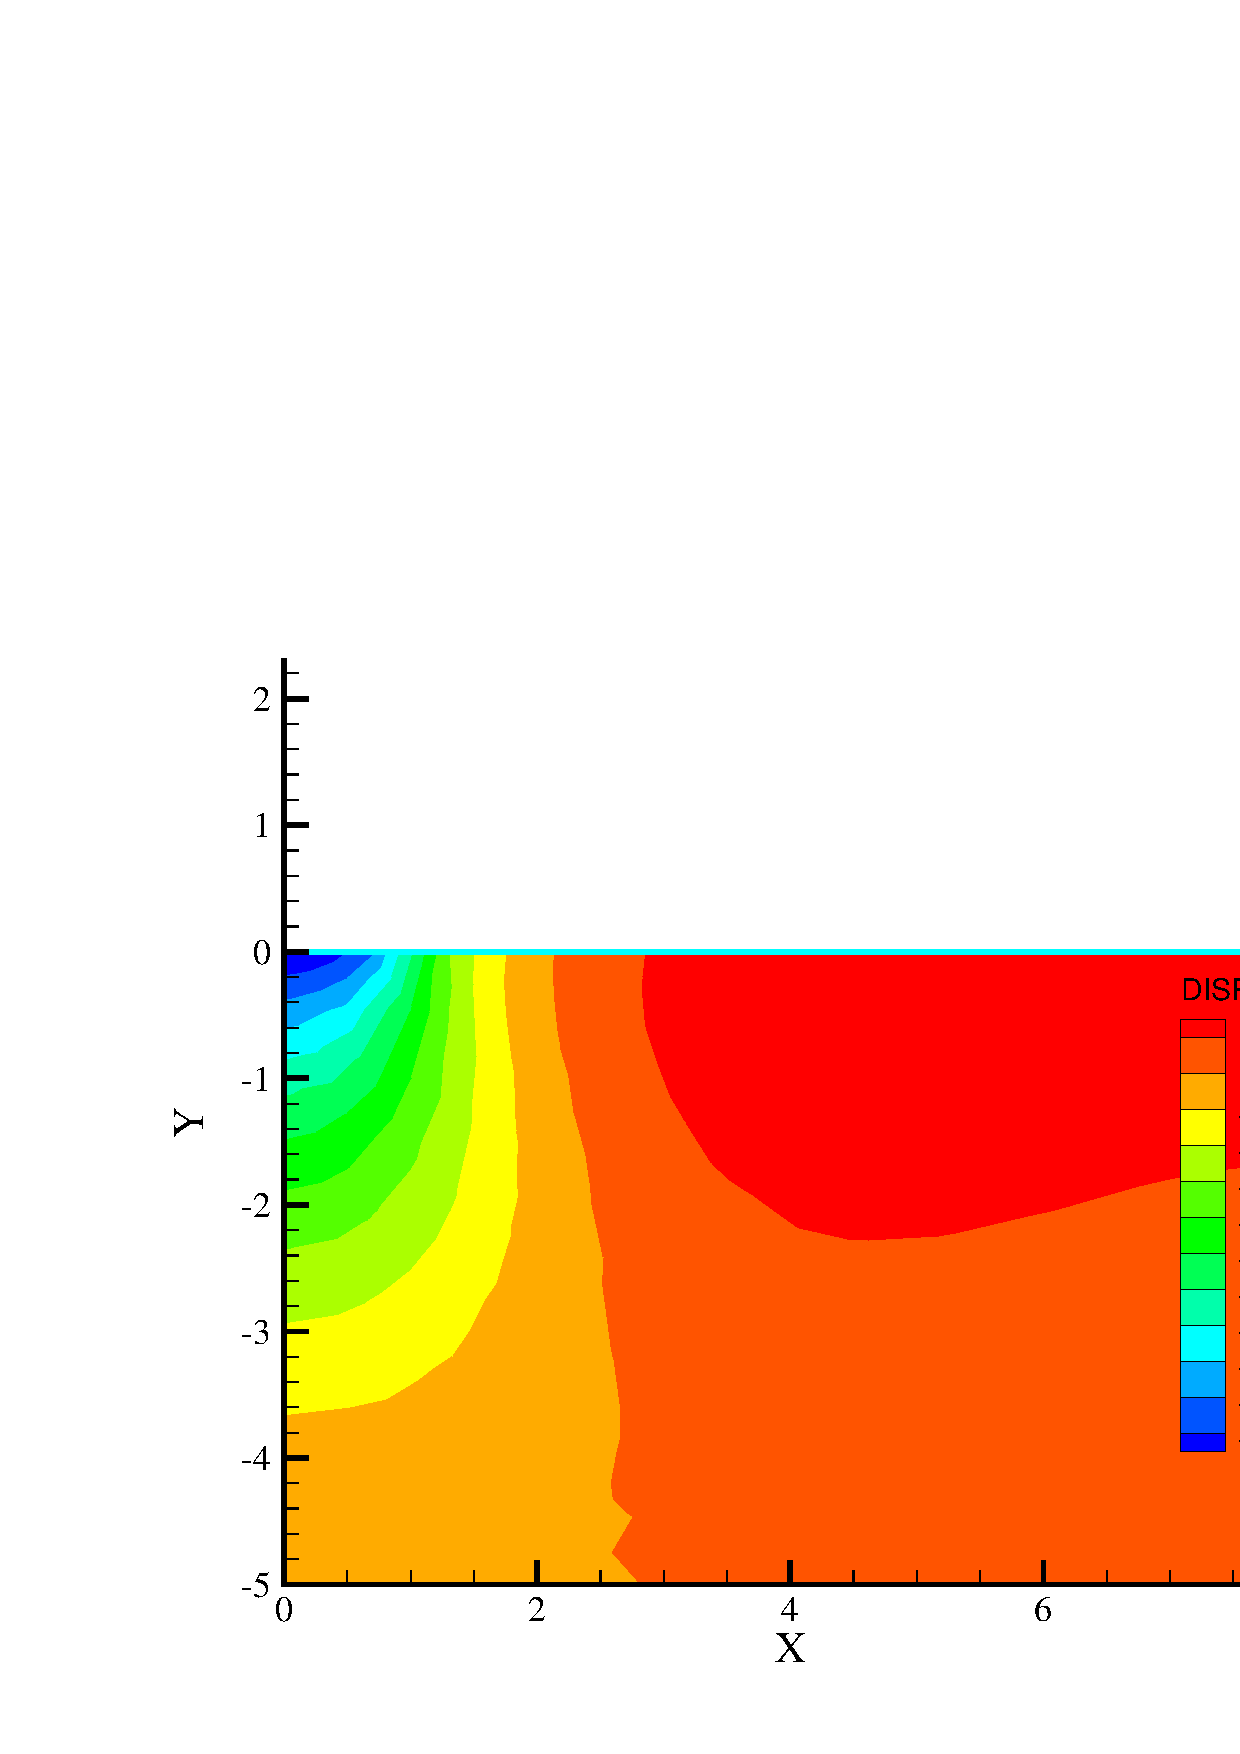
\includegraphics[width=0.32\textwidth]{chapter_14/figures/fig_14_1_10_a}
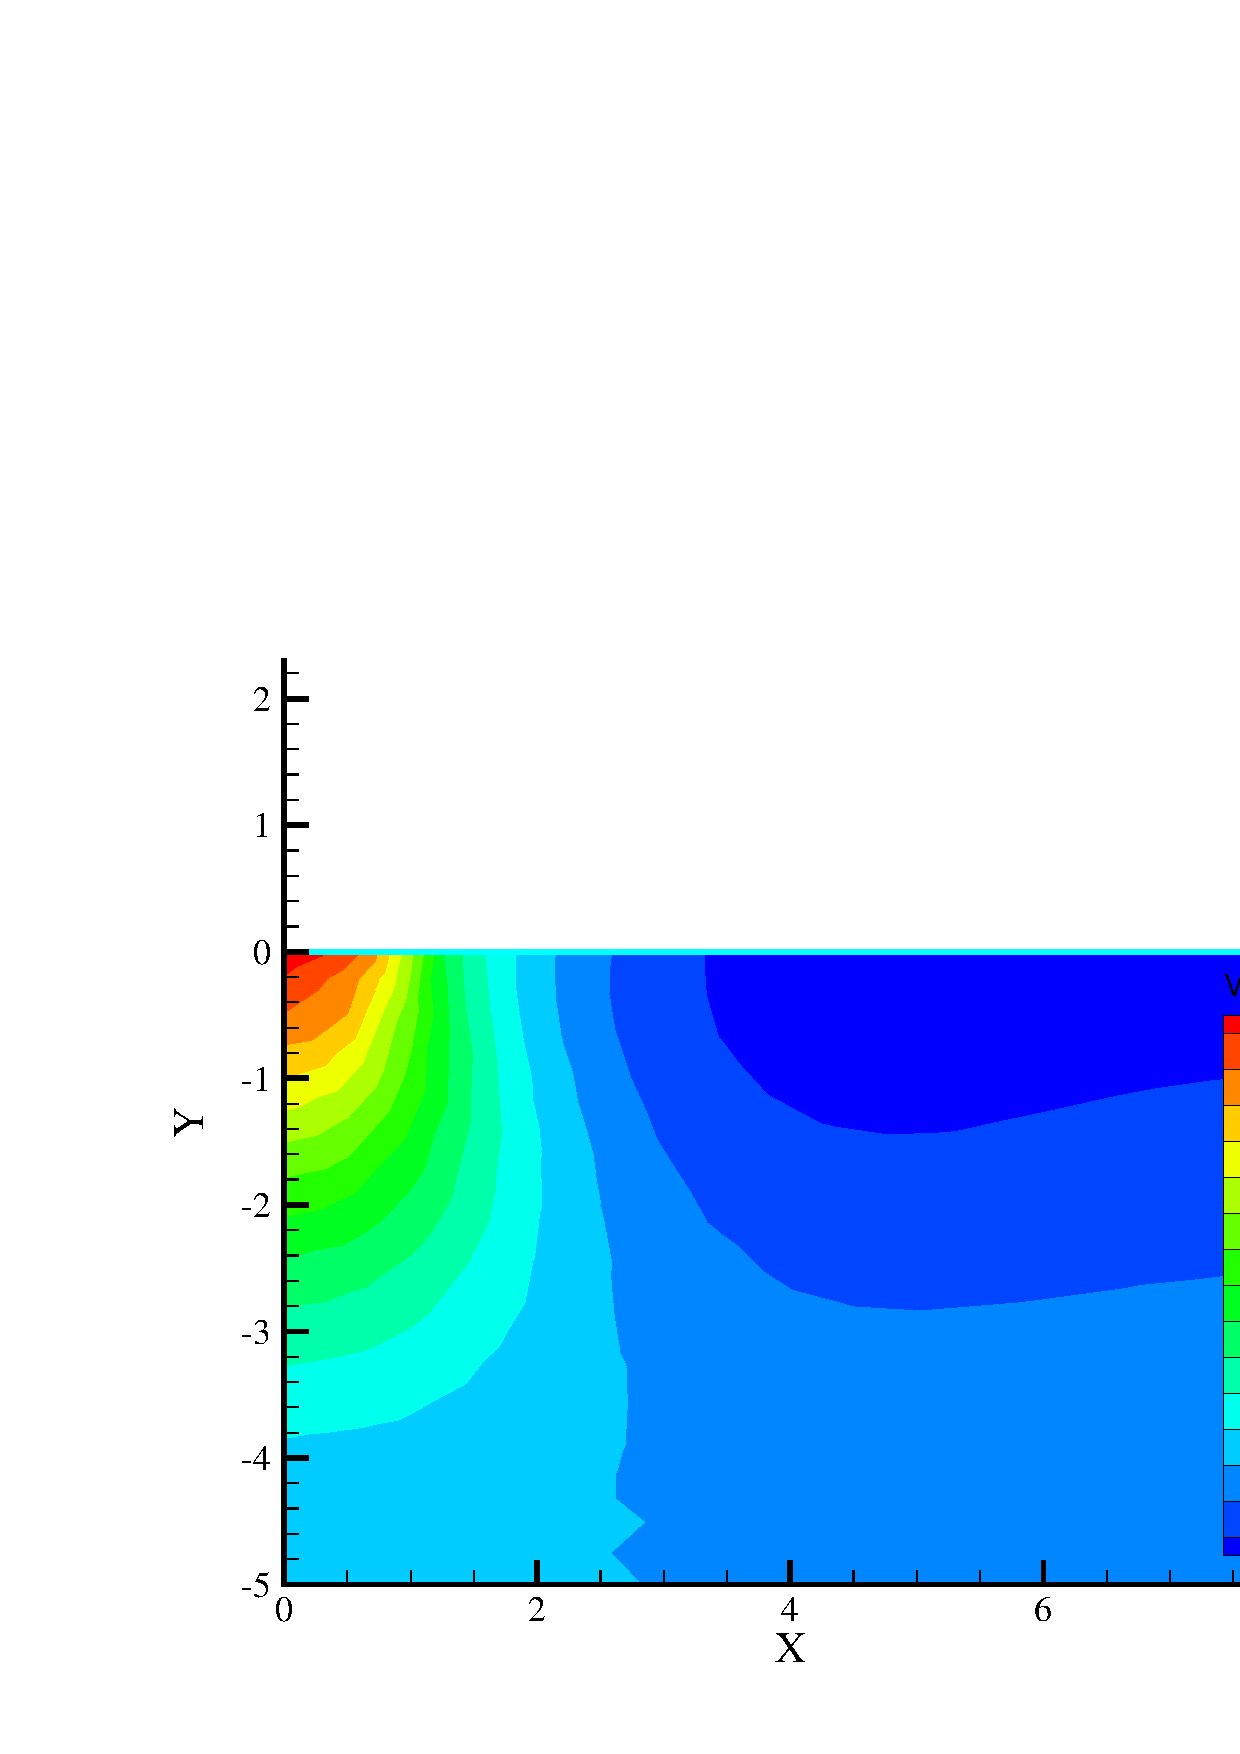
\includegraphics[width=0.32\textwidth]{chapter_14/figures/fig_14_1_10_b}
\includegraphics[width=0.32\textwidth]{chapter_14/figures/fig_14_1_10_c}
\end{center}
\caption{Displacement, its rate and acceleration: vertical component}
\label{fig_dynHM3}
\end{figure}
\begin{figure}[!htb]
\begin{center}
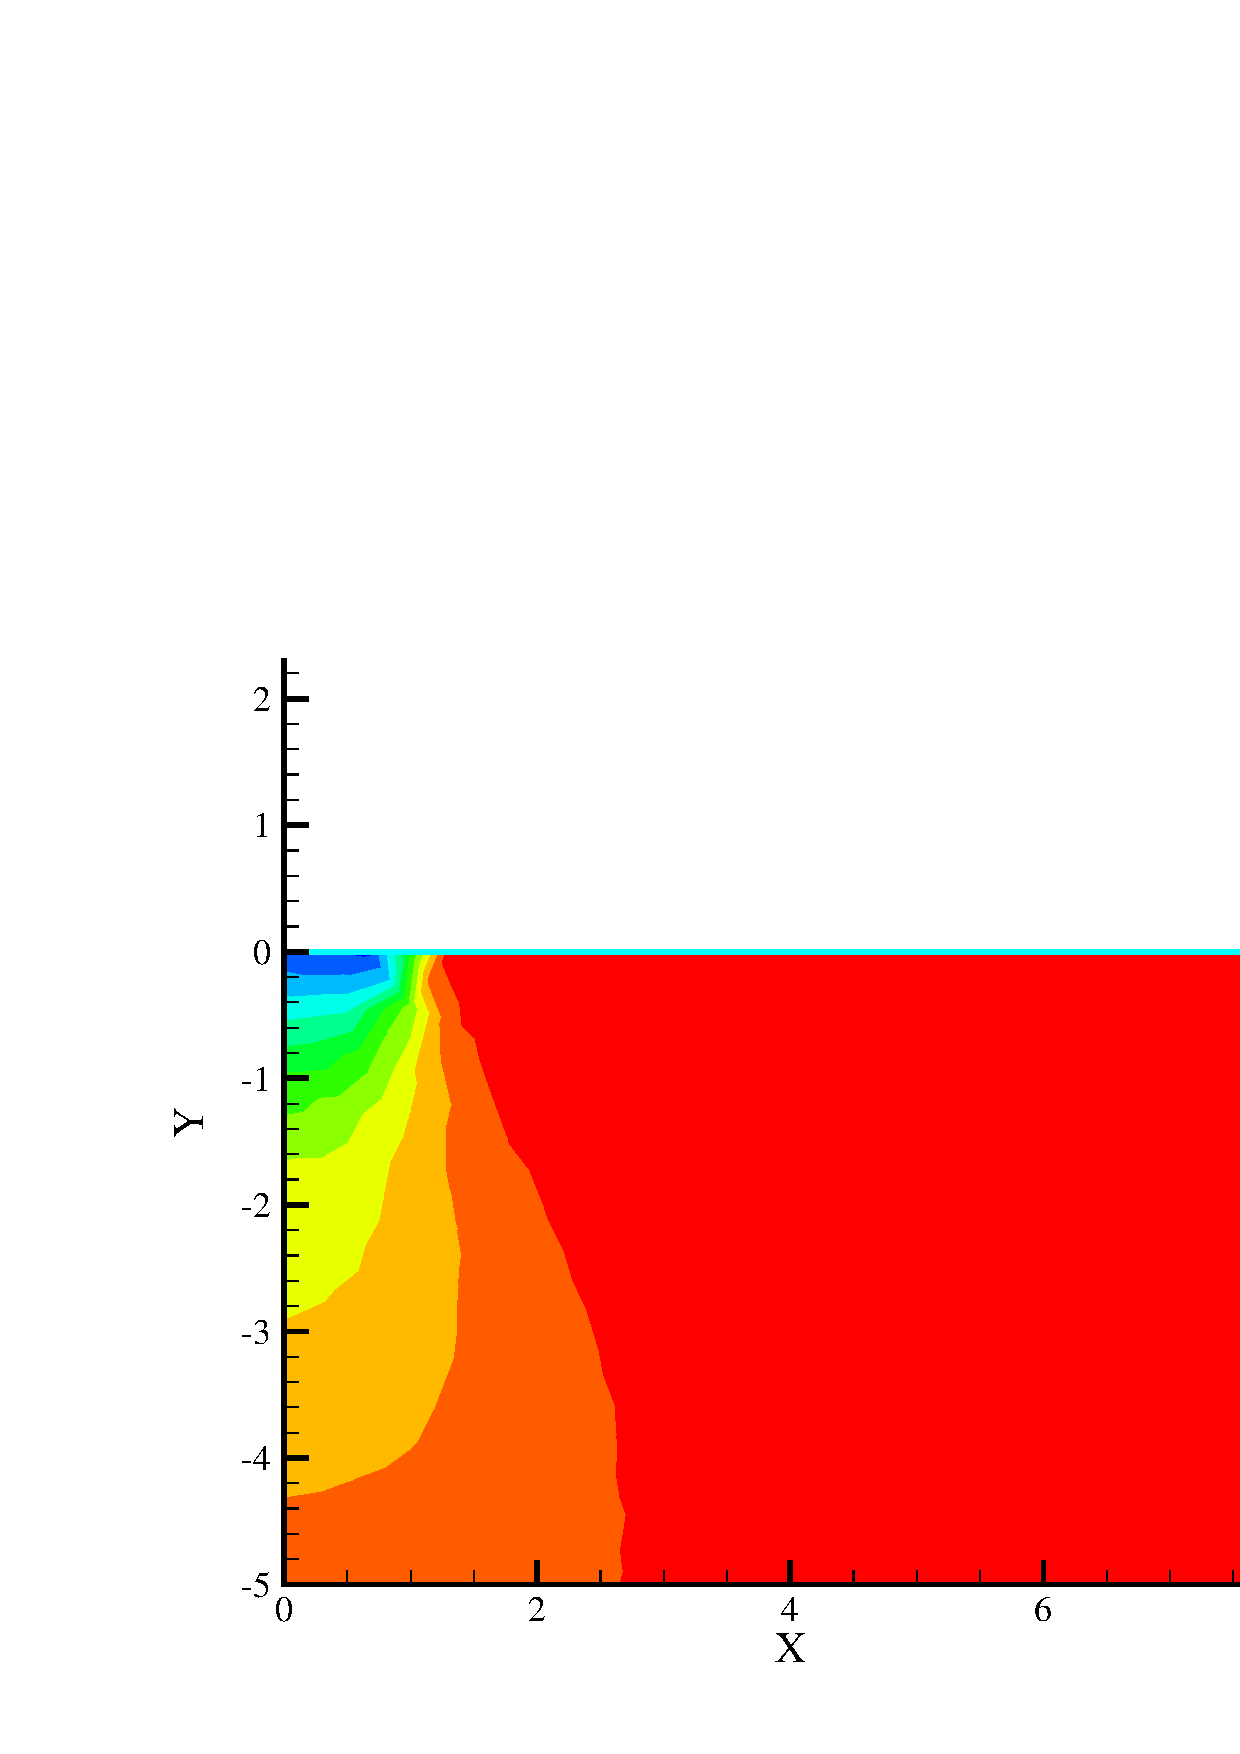
\includegraphics[width=0.5\textwidth]{chapter_14/figures/fig_14_1_11}
\end{center}
\caption{Vertical stress.}
\label{fig_dynHM4}
\end{figure}